% Lecture date: 04/29/2019, part two
% Authors: Ulzee An, David Martuscello, Xintian Han (editor)
% Time interval: 01:05:00 - 02:00:00
\chapter{Self-supervised Learning}
\section{Next Steps in AI}

\begin{table}
\begin{center}
\begin{tabular}{ |c||c| } 
 \hline
 What we can have: & What we cannot have (yet): \\ 
 \hline
 \hline
 Safer cars, autonomous cars & Machines with common sense \\ 
 Better medical image analysis & Intelligent personal assistants \\ 
 Personalized medicine & "Smart" chatbots \\
 Adequate language translation & Household robots \\
 Useful but stupid chatbots & Agile and dexterous robots \\
 Information search, retrieval, filtering & Artificial General Intelligence (AGI) \\
 (many more industry applications ...) & \\
 \hline
\end{tabular}
\caption{Professor LeCun notes several areas enabled by modern approaches in AI and others where AI falls short.}
\end{center}
\end{table}

\subsection{Defining "real" AI}

Let us consider an anecdote. Suppose a driver is steering his car alongside a cliff. Human drivers would not consider driving off the cliff to an obvious demise. 
This much foresight is clear to drivers regardless of their driving expertise. Instinctual behavior may be innate or acquired, but our ability to avoid certain doom is certainly in-place far before we even grab the steering wheel. 
Where RL agents must constantly drive off the cliff to experience its consequences, we demonstrate "common-sense" which is crucial in picking up new skills allowing most people to learn to drive in less than $36$ hours and fly a plane in similar time without catastrophic accidents.

The term Artificial General Intelligence (AGI) is discussed in this context, where an ideal AI system should be adaptable to general tasks much like humans. However, the premise that natural agents such as humans are general is highly debatable. Most biological systems are highly specialized but demonstrate remarkable flexibility within their world function. In this section "common-sense" is framed as a prediction-feedback mechanism of world dynamics and how such module can be implemented and trained.

\subsection{Lessons from Biology}

\begin{figure}
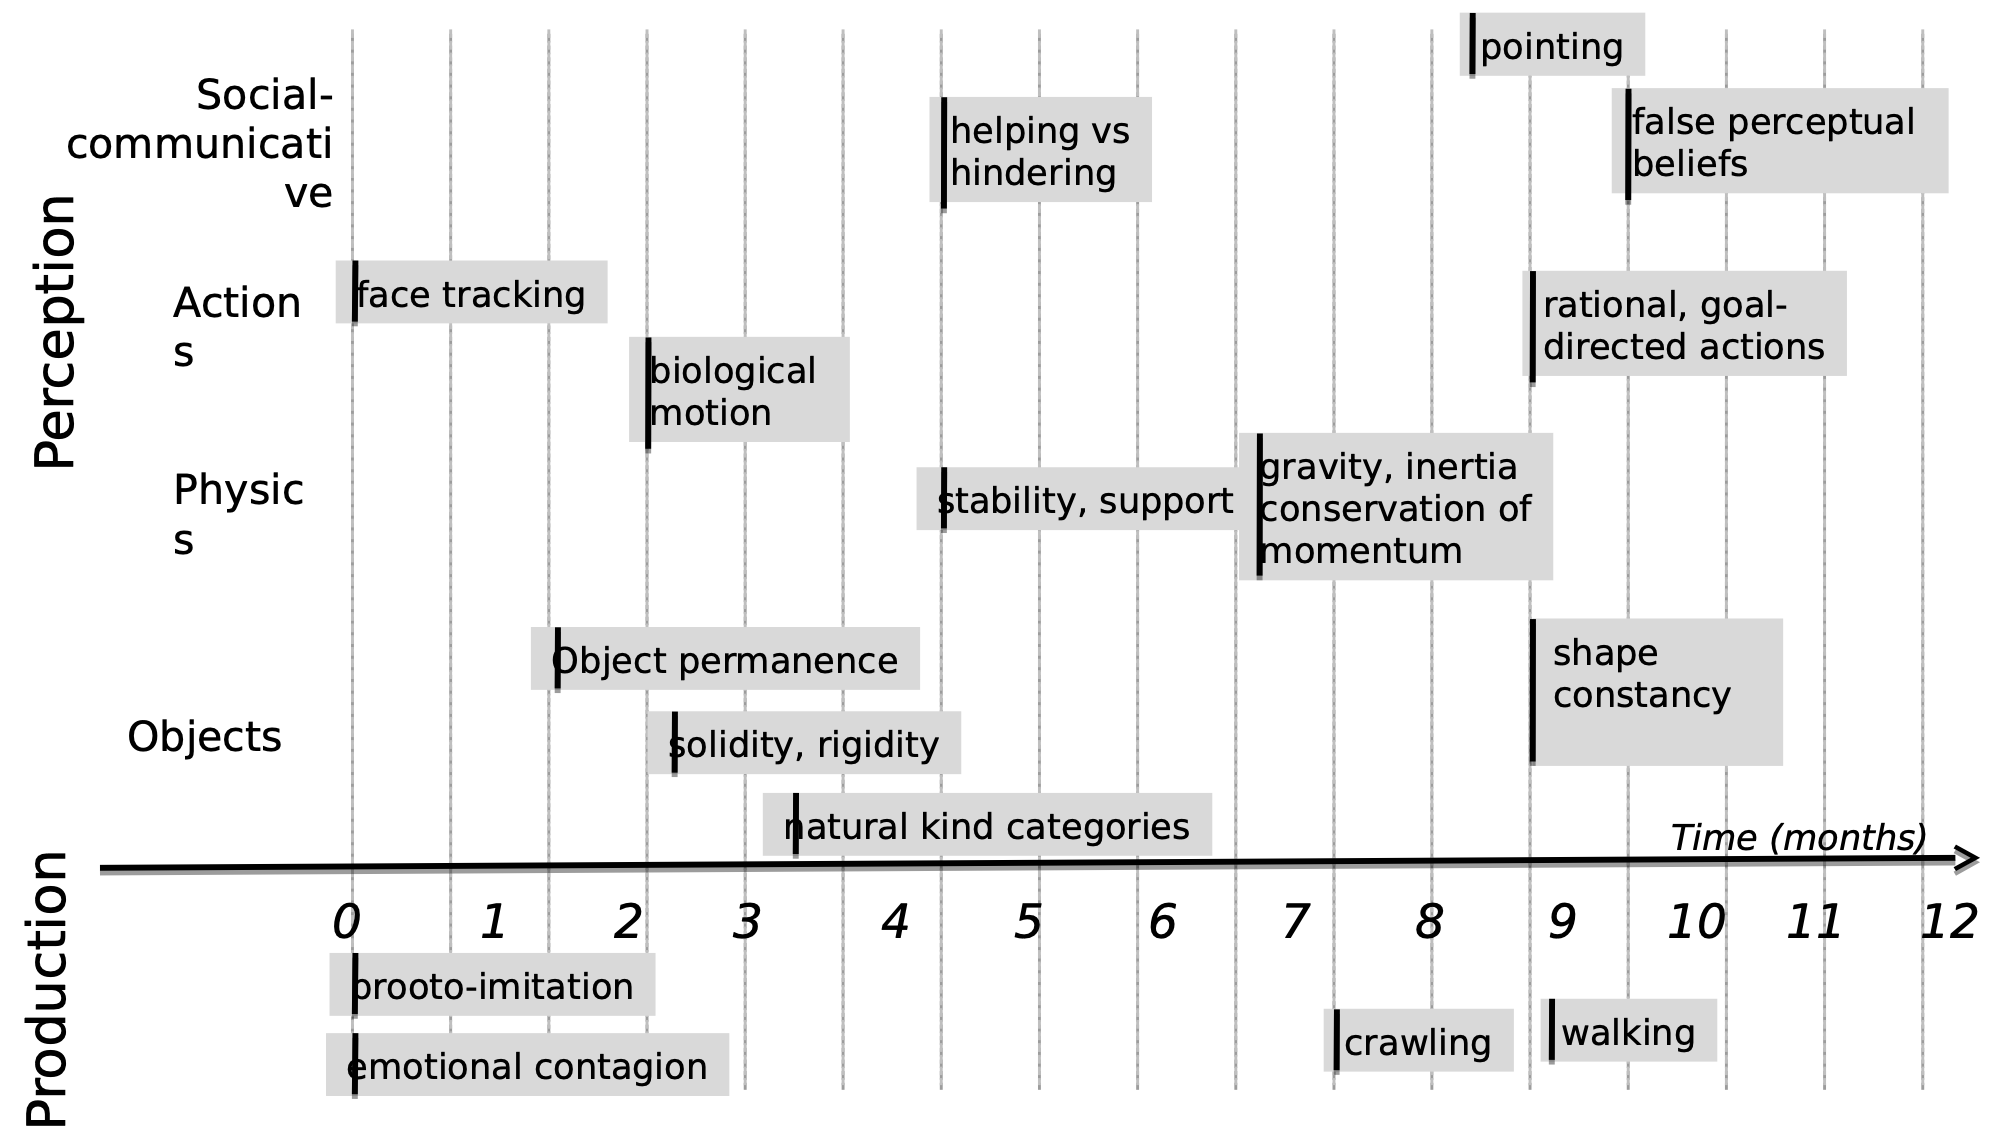
\includegraphics[width=\linewidth]{figs/baby.png}
\centering
\caption{Approximate time in months since birth when babies are shown to demonstrate awareness of worldly properties.}
\label{fig:baby}
\end{figure}

Behavioral scientists discovered that infants acquire a robust knowledge of the physical world within their first twelve months. 
There are several takeaways from this observation. 

First, babies are seldom subject to supervised learning scenarios which implies that the bulk of learning is through observation. 
Second, events which violate the developing world model cause distress in the form of surprise or fear. 
This suggests humans constantly predict expected outcomes with their world model starting from birth such that less and less outcomes appear unexpected as we age. 

While adults may be fooled by sophisticated magic tricks, babies are amused far easily playing \textit{Peak-a-boo} because they have not yet fully grasped object permanence. For similar reasons, primates can be cajoled to express strong reaction to magic tricks while distant mammals express decreasing interest.

\section{Self-Supervised Learning}

\subsection{Forms of SSL}

Through anecdotal cases and biological evidence, self-supervised learning has been theorized as a necessary step in building highly adaptable agents. 
Self-Supervised Learning (SSL) proposes a means of leveraging vast amounts of unlabelled data to learn physical dynamics of the world which is crucial in most perceptual tasks. 

SSL takes several forms and is best explained in the domain of video. Video data captures the interaction between physical objects in the world and an agent predicting any part of the video against itself must encode its relevant physical properties. The most powerful aspect of SSL on video is that the prediction task can be sliced a number of ways with minimal effort and no additional labelling step.

\begin{figure}
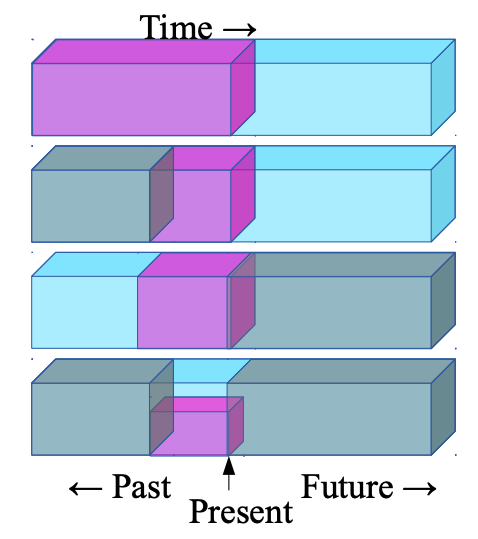
\includegraphics[width=0.5\linewidth]{figs/ssl_types.png}
\centering
\caption{Various types of SSL possible on video-like data.}
\label{fig:ssl_types}
\end{figure}

\textbf{Figure \ref{fig:ssl_types}} shows given a single stream of video, one may try to (1) predict past frames before a certain time, (2) predict a window of frames in the past, (3) predict a window of frames given past and known future frames, and (4) predict a held-out portion of such window. 

\subsection{Current Approaches}

The concept of SSL has been explored in terms of embedding methods for language and images. 
A language embedding serves a general purpose of a latent representation of words and methods such as Word2Vec, FastText, and BERT have gained popularity. 
BERT shares many similarities to SSL such that known words are withheld and predicted during training, but this method has been found to perform insufficiently for images. 
Image completion models exist, but image embedding does not reach the versatility of word embedding for many reasons, one of which is that words in a language are finite while the full distribution of image is not tractable.

In general, we take away that much work is to be done in learning which is not supervised nor reinforced. Professor LeCun hypothesizes that the "Next revolution will not be Supervised."

\section{Learning Predictive Models of the World}

Common sense requires a model of the world. In order to take actions that incorporate common sense, it is important to be able to predict the consequences of these actions. In human brains, the basal ganglia serves this purpose by providing us with a simplification of the entire state of the brain into happy or not happy. 

One of the ways that this can be implemented in a machine learning context is using an actor-critic model. A world simulation serves as a playground for the actor to experiment with various actions. The critic observes the state of this simulation and the state of the actor to determine the predicted cost of a particular action.

\begin{figure}[!ht]
\centering
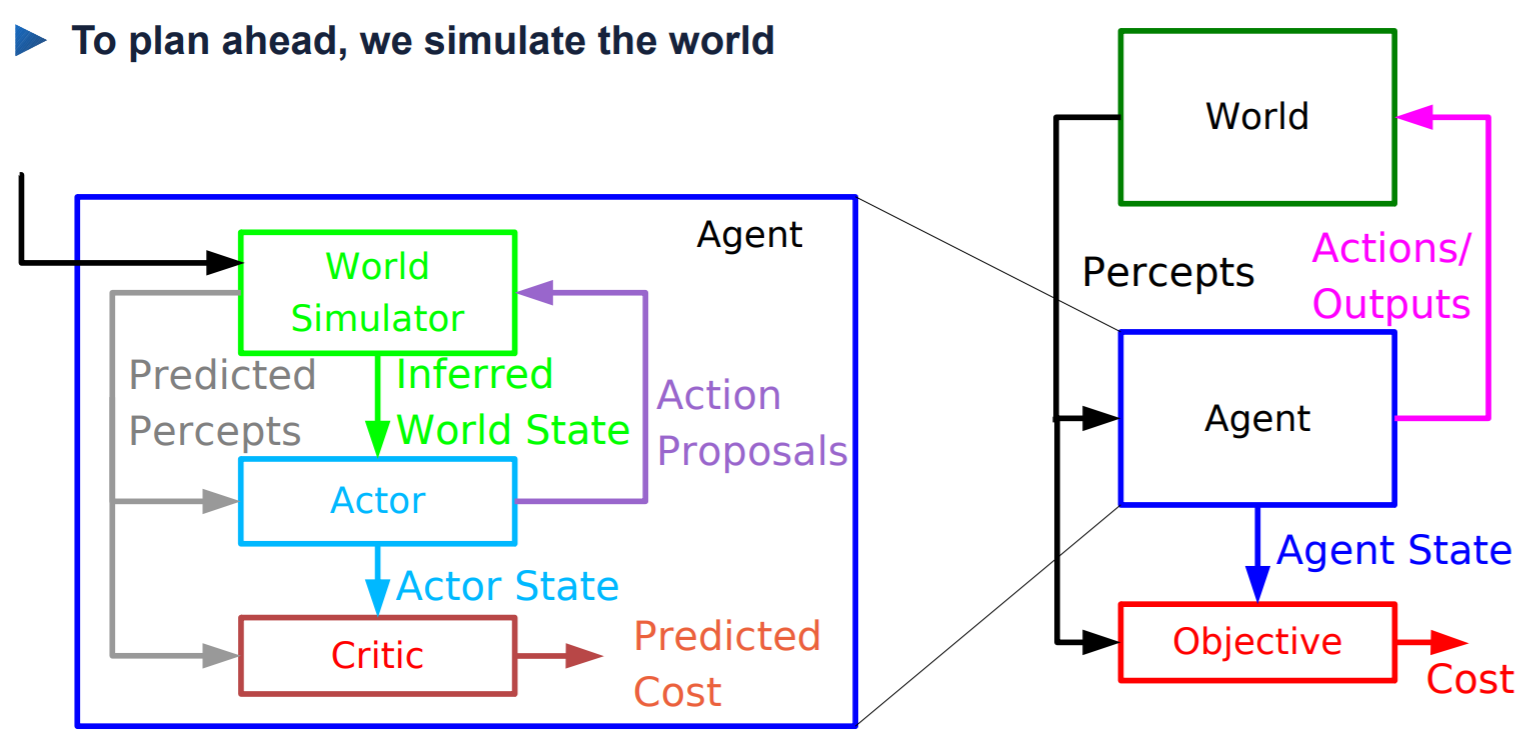
\includegraphics[scale=0.4]{figs/agent1.PNG}
\caption{Actor-Critic Model with World Simulator}
\label{fig:agent}
\end{figure}

This approach has some advantages over the alternative approach of Reinforcement Learning.
The main criticism of reinforcement learning is that the objective is not differentiable. If we can make the objective differentiable we can simply compute the ideal answer by backpropagating through it.

\section{Model Predictive Control}

Model Predictive Control is using your model of the world to predict the consequences of your actions and figure out which action optimizes the expected objective.


There are several reasons why we cannot have a perfect model of the world.

\begin{itemize}
	\item We may not have perfect perception of the world (measurement error)
	\item The world is complicated in comparison to our model
	\item Only a small slice of the world can be simulated and the world contains external influences from outside that slice.
\end{itemize}

One example of this uncertainty can be observed by setting a pen upright on a desk and releasing it to see where it falls. There is uncertainty inherent in this prediction because the pen can fall in any direction. However, it is possible to predict that the pen will fall outwards from the starting point (See Figure 2). In this case, the training samples are merely representatives of a whole set of possible outputs, which is called invariant prediction. 

\begin{figure}[!ht]
\centering
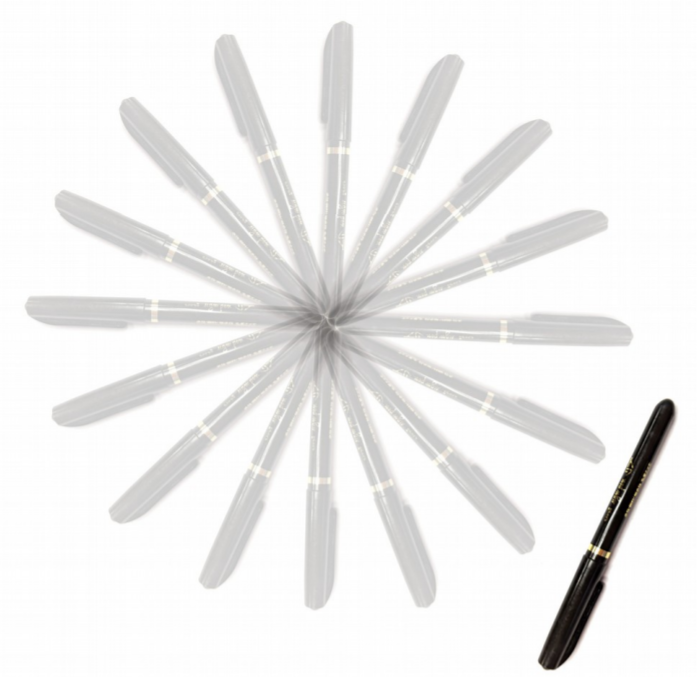
\includegraphics[scale=0.4]{figs/Pen.PNG}
\caption{Invariant Prediction of a Pen}
\label{fig:pen}
\end{figure}

One way to model this problem is by representing each observation as a sample from a  distribution of possible positions of the pen. These possible positions define a manifold in the feature space. The objective should be defined so that predictions far away from this manifold will be penalized. Generative Adversarial Networks (GANs) solve this problem by using two neural networks in sequence. The Generator network will generate a sample and the Discriminator network will try to determine if the sample lies on the manifold or not. 

The true goal of our model is to generate predictions that are plausible. Even if they are quite different from the samples we have seen, the goal is that they lie on the same manifold as those samples. This model can be represented as an energy function as shown in \cite{zhao2016energy}. The error will be backpropagated through the discriminator to update the weights of the generator to produce examples that will produce low energy.

\section{Self Supervised Forward Models of Control}

This can be applied to the problem of controlling a car in a highway of other cars. The model needs to predict where each car will move, in order to avoid a collision. A deterministic model will predict a blurry location for each car because it takes the average of all the positions that the car could move to. This is another instance of invariant prediction.

The model formulation starts with a predictor network that generates a representation of the state of the environment. This state is then combined with some action taken by the controller. The decoder network then generates a prediction of what will happen given the current state and action. In order to prevent the "blurry" results described above, we need to augment the input to the model with some latent variable ($z$) as a predictor. $z$ represents the uncertainty of the future. Changing $z$ will result in different representations for the environment, effectively selecting different scenarios for our model to learn. $z$ is generated using an "encoder" network which uses information from the past (input) and the future (target). Noise and "dropout" functionality are added to limit the amount of information from the target that is provided to our model. This encourages the model the learn the ideal action without relying to heavily on the target information.

\begin{figure}[!ht]
\centering
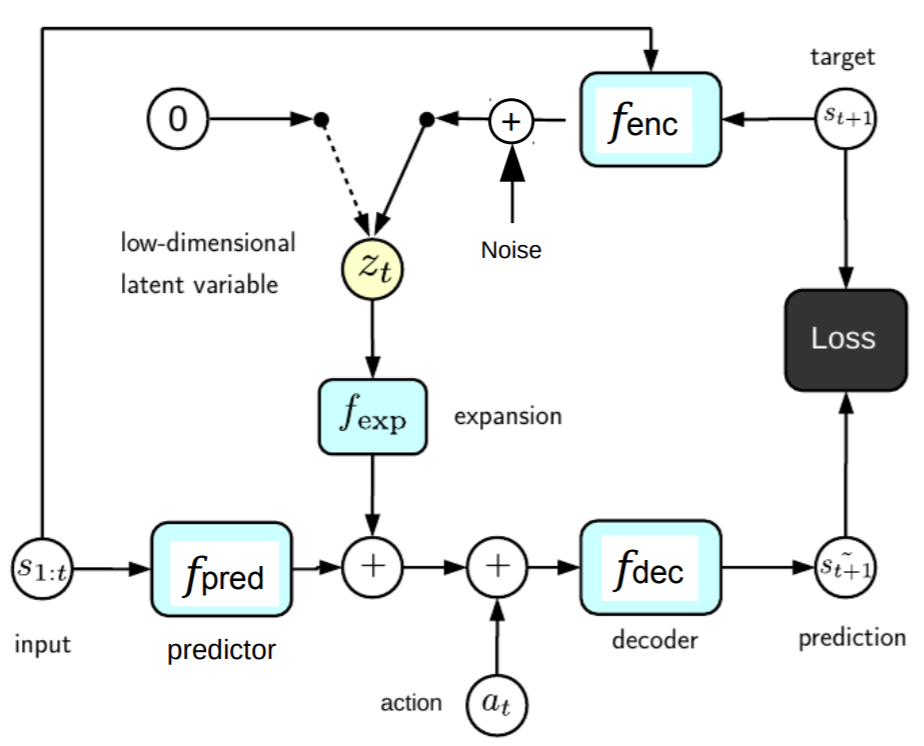
\includegraphics[scale=0.4]{figs/Model.PNG}
\caption{The predictor and decoder act as a deterministic model to generate a prediction (Bottom). The decoder and encoder act as a variational autoencoder to generate the latent variable $z$ (Right).
}
\label{fig:model}
\end{figure}